\documentclass[12pt]{article}
\usepackage[spanish,es-nodecimaldot]{babel}
\usepackage[utf8]{inputenc}
\usepackage[T1]{fontenc}
\usepackage{newtxtext,newtxmath}
\usepackage[letterpaper,margin=1in]{geometry}
\usepackage{setspace,graphicx,booktabs,array,float,url,caption,hanging}
\usepackage[hidelinks]{hyperref}
\usepackage{fancyhdr}
\usepackage{tikz}
\usetikzlibrary{positioning,arrows.meta}
\setstretch{2}
\setlength{\parindent}{0.5in}
\setlength{\parskip}{0pt}
\setlength{\headheight}{15pt}
\pagestyle{fancy}\fancyhf{}\fancyhead[R]{\thepage}\renewcommand{\headrulewidth}{0pt}
\captionsetup{font=small,labelfont=bf,labelsep=period}
\newcommand{\student}{Karen Sofía Delgado Calderón}
\newcommand{\repo}{\href{https://github.com/sofiadelcal/karen-transformers-pronostico-73178}{repositorio público}}
\newcommand{\colab}{\href{https://colab.research.google.com/github/sofiadelcal/karen-transformers-pronostico-73178/blob/main/Karen_Transformers_Pronostico.ipynb}{cuaderno reproducible en Colab}}

\begin{document}
\begin{titlepage}
\thispagestyle{empty}\centering
\vspace*{1.2in}
{\bfseries Pronóstico de demanda horaria a corto plazo con atención temporal y Transformer causal\par}
\vspace{1.15in}
\student\par
Universidad de Cundinamarca\par
Especialización en Inteligencia Artificial\par
Deep Learning -- Conceptos\par
R2-A3-S12: Transformers\par
Docente de la asignatura\par
19 de noviembre de 2026\par
\vfill
\end{titlepage}
\setcounter{page}{2}

\begin{center}\textbf{Pronóstico de demanda horaria a corto plazo con atención temporal y Transformer causal}\end{center}

\section{Introducción}
Al pronosticar una serie horaria, la historia reciente puede contener varios ritmos a la vez: ciclos diarios, variaciones semanales y cambios graduales del nivel. Un modelo que mira únicamente los últimos valores puede no distinguir cuál de esos patrones resulta útil para el siguiente tramo. La atención permite ponderar observaciones de la ventana de entrada y el Transformer extiende esa idea mediante autoatención y codificación posicional (Vaswani et al., 2017).

Este informe propone un experimento reproducible de pronóstico de seis horas. Se comparan una atención aditiva temporal y un Transformer causal pequeño con dos referencias sencillas: persistencia y repetición del perfil de hace 24 horas. La señal es sintética; se diseñó para incluir ritmos diarios y semanales y un cambio suave de nivel, y no se presenta como medición de una empresa o de una persona. La pregunta que guía el análisis es concreta: ¿la atención aprendida agrega valor frente a repetir un patrón temporal conocido en este escenario didáctico?

\section{Objetivos}
El objetivo general es implementar y analizar mecanismos de atención para pronóstico de series de tiempo con TensorFlow/Keras. Se busca preparar ventanas respetando el orden cronológico, entrenar los dos modelos con validación temporal, comparar sus errores en un bloque futuro y discutir qué permiten concluir los resultados y qué queda fuera del alcance del experimento.

\section{Fundamento}
La atención escalada combina consultas, claves y valores mediante
\begin{equation}
\operatorname{Attention}(Q,K,V)=\operatorname{softmax}\!\left(\frac{QK^{\mathsf T}}{\sqrt{d_k}}\right)V.
\end{equation}
La distribución softmax asigna pesos a las posiciones y el producto con los valores forma una representación contextual. En la variante aditiva implementada, la representación del instante final actúa como consulta y se compara con cada posición anterior. El contexto resultante resume las 48 horas de historia con pesos aprendidos.

El Transformer proyecta cada observación a un espacio de 32 dimensiones, agrega embeddings posicionales y aplica autoatención multi-cabeza. La máscara causal limita cada posición a información disponible hasta ese instante. Una conexión residual, normalización y una red feed-forward transforman la secuencia; la salida del último estado produce directamente seis valores futuros. En predicción de series, estos diseños se han adaptado para capturar dependencias temporales y reducir el costo de atender secuencias largas (Zhou et al., 2021; Nie et al., 2023). El ejercicio usa una arquitectura pedagógica, no una reproducción completa de Informer o PatchTST.

\section{Método}
\subsection{Señal y partición}
El cuaderno genera 1\,008 observaciones horarias mediante una suma de tendencia suave, ciclo de 24 horas, componente semanal, variación intradía y ruido gaussiano con semilla fija. A partir de la hora 670 el nivel cambia gradualmente, de modo que la prueba cubre un régimen algo distinto al inicio. La construcción deliberada de la señal ayuda a explicar sus componentes, pero también restringe cualquier generalización: un patrón sintético no sustituye un conjunto de demanda observado.

Los primeros 80\% de los puntos forman el tramo de ajuste y el último 20\% queda reservado para prueba. La media y desviación para normalizar se calculan solo con el tramo de ajuste. Cada ejemplo usa 48 horas y predice el bloque de seis horas siguiente; las ventanas avanzan seis pasos para evitar que los objetivos de evaluación se repitan. El 15\% final de las ventanas de entrenamiento se reserva para validación. No se aleatorizan observaciones entre pasado y futuro.

\subsection{Modelos y comparación}
La atención aditiva proyecta la historia a 32 dimensiones, aprende una distribución de pesos en el eje temporal y genera seis pronósticos desde el contexto ponderado. El Transformer tiene cuatro cabezas de atención, dimensión de modelo 32 y máscara causal. Ambos se optimizan con Adam y pérdida cuadrática, con tamaño de lote 32, máximo de 50 épocas y detención temprana si la pérdida de validación no mejora durante siete épocas.

Se fijan tres semillas (7, 23 y 58) para estimar la variación por inicialización. Las referencias no entrenables repiten el último valor observado o reutilizan los seis valores del mismo intervalo del día anterior. Se reportan MAE y RMSE en la escala original. Las métricas se calculan sobre todas las horas pronosticadas del bloque de prueba, no sobre datos de entrenamiento. El cuaderno guarda resultados por semilla, pronósticos, resumen y figuras para que la tabla pueda auditarse.

\begin{figure}[H]
\centering
\begin{tikzpicture}[node distance=0.55cm and 0.65cm,
  b/.style={draw=black!55,rounded corners,align=center,minimum height=0.85cm,text width=2.15cm,fill=teal!7,font=\small},
  m/.style={b,fill=orange!12}, a/.style={-{Latex[length=2mm]},thick,draw=black!65}]
\node[b] (s) {Señal horaria\\1\,008 puntos};
\node[b,right=of s] (w) {Ventana de 48 h\\horizonte de 6 h};
\node[b,right=of w] (p) {Corte temporal\\80\% / 20\%};
\node[m,right=1cm of p,yshift=.62cm] (aa) {Atención\\aditiva};
\node[m,right=1cm of p,yshift=-.62cm] (tr) {Transformer\\causal};
\node[b,right=1cm of aa,yshift=-.62cm,fill=green!10] (e) {MAE y RMSE\\contra referencias};
\draw[a] (s)--(w); \draw[a] (w)--(p);
\draw[a] (p.east)--++(.35,0)|-(aa.west); \draw[a] (p.east)--++(.35,0)|-(tr.west);
\draw[a] (aa.east)--(e.west); \draw[a] (tr.east)--(e.west);
\end{tikzpicture}
\caption{Secuencia de preparación, modelado y evaluación planteada para la práctica.}
\end{figure}

\begin{figure}[H]
\centering
\IfFileExists{resultados/serie_particion.png}{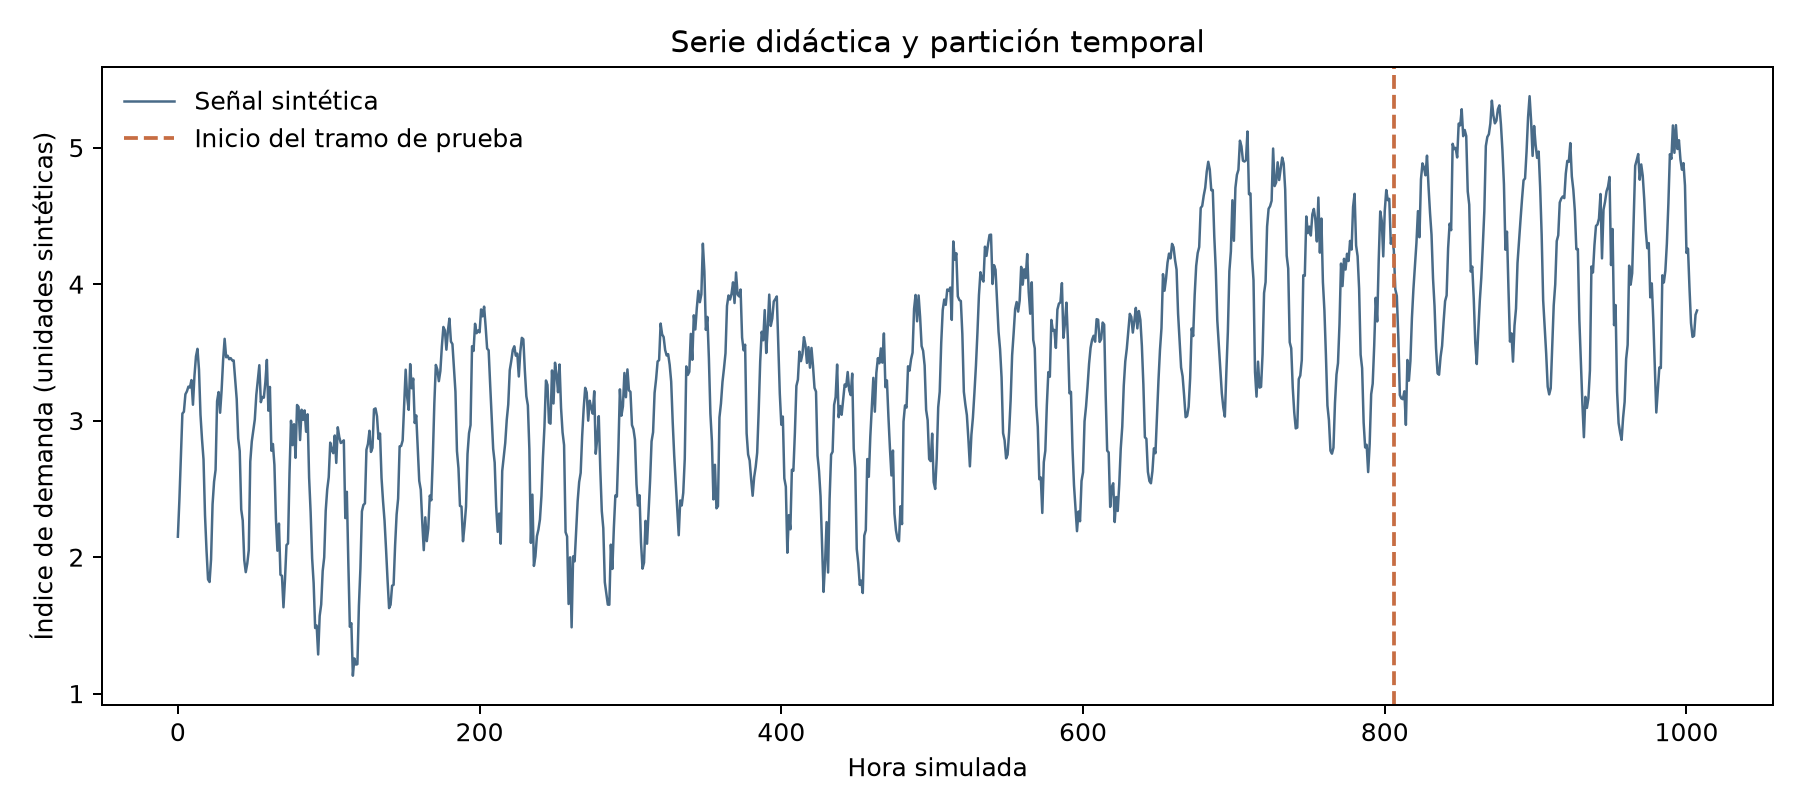
\includegraphics[width=.9\linewidth]{resultados/serie_particion.png}}{\fbox{La figura se crea al ejecutar el cuaderno.}}
\caption{Señal didáctica y separación cronológica prevista.}
\end{figure}

\begin{figure}[H]
\centering
\IfFileExists{resultados/comparacion_rmse.png}{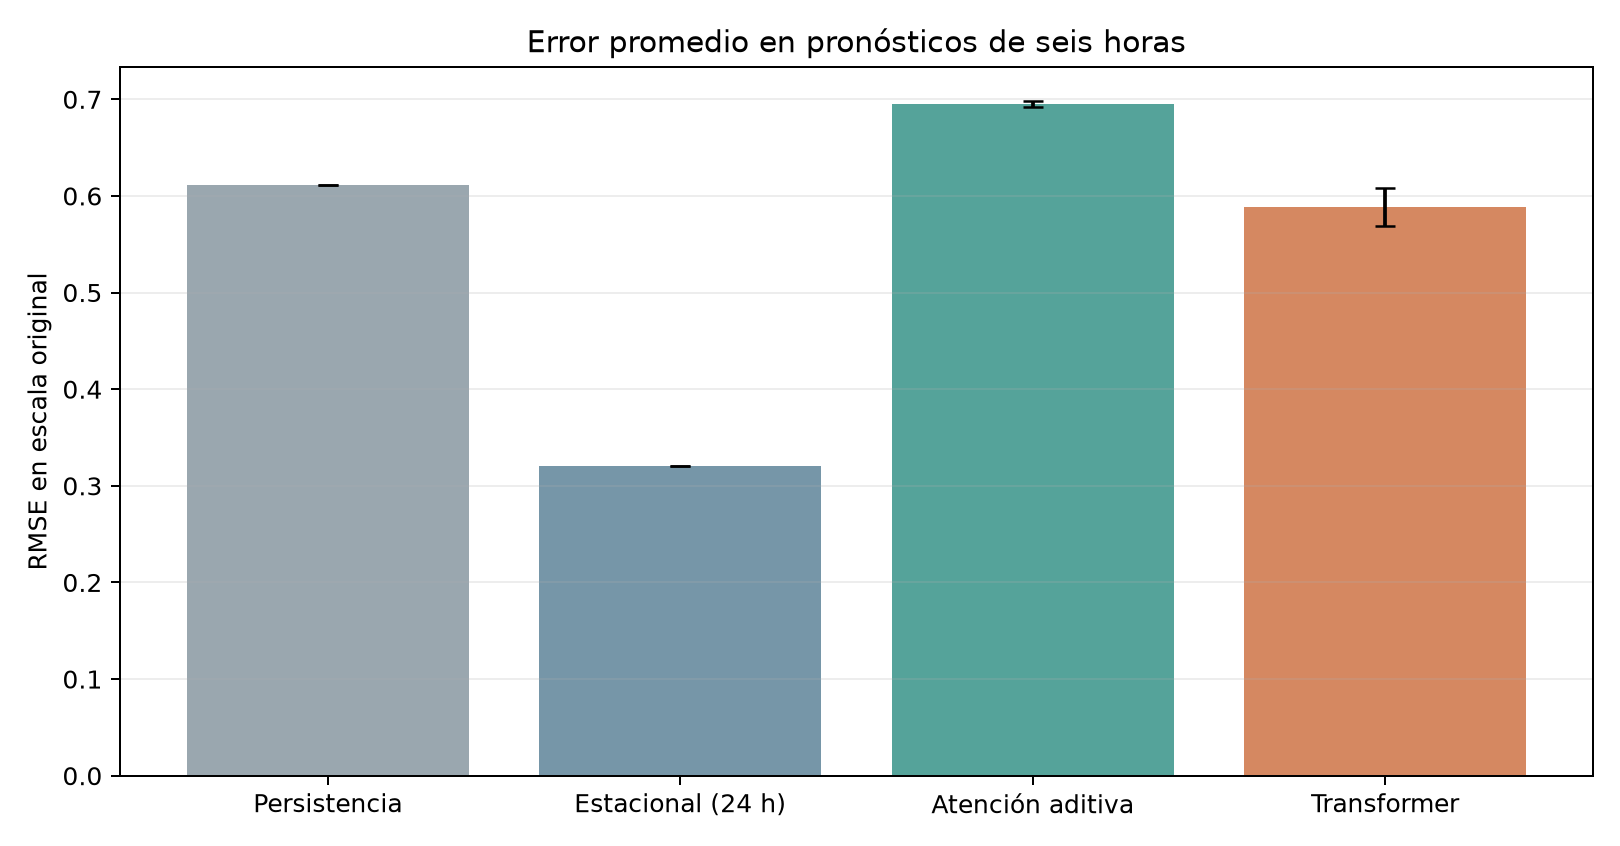
\includegraphics[width=.88\linewidth]{resultados/comparacion_rmse.png}}{\fbox{Ejecute el cuaderno para generar la comparación.}}
\caption{RMSE en el bloque de prueba; las barras de error muestran la desviación estándar entre semillas para los modelos entrenables.}
\end{figure}

\section{Resultados y análisis}
La ejecución del cuaderno en Google Colab (TensorFlow 2.21.0) produjo 33 ventanas de prueba y entrenó cada arquitectura con tres inicializaciones. La tabla presenta el promedio y la desviación estándar entre semillas; para los métodos de referencia, que no se entrenan, se informa una sola evaluación. Los errores se expresan en las unidades sintéticas de la señal.

\begin{table}[H]
\centering
\caption{Métricas del bloque de prueba para pronósticos a seis horas}
\begin{tabular}{lcc}
\toprule
Modelo & MAE (M \(\pm\) DE) & RMSE (M \(\pm\) DE) \\
\midrule
Persistencia & 0.5068 (--) & 0.6112 (--) \\
Estacional (24 h) & 0.2680 (--) & 0.3201 (--) \\
Atención aditiva & 0.5963 (0.0091) & 0.6952 (0.0031) \\
Transformer causal & 0.5041 (0.0167) & 0.5885 (0.0199) \\
\bottomrule
\end{tabular}
\end{table}

La referencia estacional obtuvo el menor error (MAE = 0.2680; RMSE = 0.3201). El Transformer quedó cerca de persistencia en MAE y tuvo un RMSE algo menor (0.5885 frente a 0.6112), pero ambos errores fueron claramente superiores a los de la referencia estacional. La atención aditiva presentó los errores más altos. Por tanto, con esta señal y configuración, el experimento no muestra una ventaja predictiva de los modelos aprendidos frente al patrón de 24 horas. El resultado es útil porque evita concluir que una arquitectura más compleja mejora automáticamente un pronóstico.

La variación entre semillas fue pequeña para la atención aditiva y mayor para el Transformer, aunque no cambió el orden general frente a la referencia estacional. La repetición diaria funciona bien porque la señal fue construida con un ciclo de 24 horas; esta coincidencia favorece deliberadamente a esa referencia. En una serie real con cambios de régimen, datos faltantes o ciclos irregulares, el resultado podría ser distinto. Los pesos de atención sirven para inspeccionar qué posiciones recibieron mayor ponderación, pero no prueban causalidad ni explican por sí solos el comportamiento del modelo.

La tabla detallada por semilla, el resumen JSON y la gráfica de RMSE se incluyen en el repositorio para facilitar la comprobación de los valores reportados.

\section{Discusión y limitaciones}
La comparación separa explícitamente el efecto de aprender atención del de usar un patrón horario conocido. También evita una conclusión basada solo en complejidad: persistencia y estacionalidad son controles mínimos que un sistema aprendido debe superar para justificar su costo. La literatura de pronóstico con Transformers estudia secuencias y conjuntos mucho más amplios; los resultados publicados de Informer y PatchTST motivan las decisiones arquitectónicas, pero no predicen el resultado de esta señal (Zhou et al., 2021; Nie et al., 2023).

La principal limitación es que la señal no procede de consumo eléctrico medido. Además, hay un solo horizonte, una sola partición y tres inicializaciones. No se realiza validación de origen rodante ni ajuste exhaustivo de hiperparámetros. En una aplicación real habría que documentar la procedencia y unidades de los datos, evaluar varios periodos, incluir un protocolo de validación temporal y comprobar el desempeño por hora y por régimen.

\section{Conclusiones}
La práctica permitió implementar atención aditiva y autoatención causal y compararlas en una predicción multi-horizonte con separación cronológica. En esta ejecución, la referencia estacional superó a las dos arquitecturas aprendidas; el Transformer mejoró ligeramente el RMSE de persistencia, mientras que la atención aditiva no superó ninguna de las dos referencias. La conclusión se limita a la señal sintética, un horizonte, una partición y tres inicializaciones; no se extrapola a demanda real.

\section*{Código y reproducibilidad}
El cuaderno del proyecto puede abrirse en \colab. El repositorio público contiene el código, los resultados de la corrida documentada y el informe: \repo. Para reproducir localmente, instalar \path{requirements.txt} y ejecutar \path{python experimento_transformers.py}. La señal es sintética y las cifras corresponden a la configuración indicada en el método.

\section*{Referencias}
\begin{hangparas}{0.5in}{1}
Nie, Y., Nguyen, N. H., Sinthong, P., \& Kalagnanam, J. (2023). A time series is worth 64 words: Long-term forecasting with Transformers. En \textit{International Conference on Learning Representations}. \url{https://openreview.net/forum?id=Jbdc0vTOcol}

Vaswani, A., Shazeer, N., Parmar, N., Uszkoreit, J., Jones, L., Gomez, A. N., Kaiser, Ł., \& Polosukhin, I. (2017). Attention is all you need. En \textit{Advances in Neural Information Processing Systems} (Vol. 30). \url{https://arxiv.org/abs/1706.03762}

Zhou, H., Zhang, S., Peng, J., Zhang, S., Li, J., Xiong, H., \& Zhang, W. (2021). Informer: Beyond efficient Transformer for long sequence time-series forecasting. \textit{Proceedings of the AAAI Conference on Artificial Intelligence, 35}(12), 11106--11115. \url{https://doi.org/10.1609/aaai.v35i12.17325}
\end{hangparas}
\end{document}
